\documentclass{X:/Documents/Coding/Latex/myassignment}
\title{Mathematical Biology Assignment 2}

\begin{document}
\maketitle
Normally I would paraphrase the  the questions, but instead I have appended the question sheet to the end
\begin{enumerate}

	%Q1
	\item 
	\begin{enumerate}
		%Q1a
		\item Given the reaction occurs stepwise
		% , and letting $n_M, n_H$ be the total number of $N$ and $M$ gates, the general reaction system is:
		% \begin{align*}
		% 	S_{i,j} \xrightleftharpoons[(i+1)\beta]{(n_{M} - i)\alpha} S_{i+1,j}\\
		% 	S_{i,j} \xrightleftharpoons[(j+1)\gamma]{(n_{H} - j)\delta} S_{i,j+1}\\
		% \end{align*}

		We have $i=0,1$ and $j=0$ so we can write the system as:
		\begin{align*}
			S_{0,j} &\xrightleftharpoons[\beta]{2\alpha} S_{1,j} \xrightleftharpoons[2\beta]{\alpha} S_{2,j}\\
			S_{i,0} &\xrightleftharpoons[\gamma]{\delta} S_{i,1}
		\end{align*}

		So the DE system is:

		\begin{align*}
			%					-> S_{10}        -> S_{01}      
			\dd{S_{00}}{t} &= - 2 \alpha S_{00} -\delta S_{00} + \beta S_{10} + \gamma S_{01} \\
			%					-> S_{11}        -> S_{00}     
			\dd{S_{01}}{t} &= - 2 \alpha S_{01} - \gamma S_{01} +\beta S_{11} + \delta S_{00} \\
			%					-> S_{20}      -> S_{00}       -> S_{11}
			\dd{S_{10}}{t} &= - \alpha S_{10} -\beta S_{10} - \delta S_{10} + 2 \beta S_{20} + 2\alpha S_{00} +  \gamma S_{11}\\
			%					-> S_{21}      -> S_{01}       -> S_{10}
			\dd{S_{11}}{t} &= - \alpha S_{11} -\beta S_{11} - \gamma S_{11} + 2 \beta S_{21} + 2\alpha S_{01} +  \delta S_{10}\\
			%
			\dd{S_{20}}{t} &= - 2\beta S_{20} - \delta S_{20} + \alpha S_{10} + \gamma S_{21} \\
			%
			\dd{S_{21}}{t} &= - 2\beta S_{21} - \gamma S_{21} + \alpha S_{11} + \delta S_{20} \\
		\end{align*}


		With the condition that 
		\[\sum_{i} \sum_{j} S_{ij} = 1\]
		Or in full
		\[S_{00} + S_{01} + S_{10} + S_{11} + S_{20} + S_{21} = 1\]


		%A1b
		\item
		Noting that $S_{ij}$ is the proportion of channels with $i$ open $m$ gates and $j$ open $h$ gates,
		\begin{align*}
			m &= \frac12 S_{10} + \frac12 S_{11} + S_{20} + S_{21}\\
			h &= S_{01} + S_{11} + S_{21}
		\end{align*}
		And taking the derivative with respect to $t$ gives
		\begin{align*}
			\odd m t &= \frac12\odd{S_{10}}{t} + \frac12\odd{S_{11}}{t} + \odd{S_{20}}{t} + \odd{S_{21}}{t}\\
			&= \frac12(- 2\alpha S_{10} -\beta S_{10} - \delta S_{10} + 2 \beta S_{20} + 2\alpha S_{00} +  \gamma S_{11})\\
			&+ \frac12(-2\alpha S_{11} -\beta S_{11} - \gamma S_{11} + 2 \beta S_{21} + 2\alpha S_{01} +  \delta S_{10}) \\
			&+ \left(- 2\beta S_{20} - \delta S_{20} + \alpha S_{10} + \gamma S_{21} \right) +  \left( - 2\beta S_{21} - \gamma S_{21} + \alpha S_{11} + \delta S_{20}\right)\\\\
			&= S_{00} \left(\alpha\right) + S_{01} \left(\alpha\right) + S_{10} \left(- \alpha - \frac12\beta - \frac12\delta + \frac12\delta + \alpha\right) + S_{11}\left(\frac12\gamma - \alpha - \frac12\beta - \frac12\gamma + \alpha\right) \\
			&+ S_{20} \left(\beta - 2 \beta - \delta +  \delta\right) + S_{21} \left(\beta +  \gamma - 2 \beta - \gamma\right)\\\\
			&= \alpha S_{00} + \alpha S_{01} - \frac12 \beta S_{10} - \beta S_{11} - \beta S_{20} - \beta S_{21}\\
			&= \alpha(S_{00} + S_{01}) - \beta (\frac12S_{10} + \frac12 S_{11} + S_{20} + S_{21})\\
			\odd mt &= \alpha(1-m) - \beta m
		\end{align*}
		By using 
		\begin{align*}
			m = \frac12 S_{10} + \frac12 S_{11} + S_{20} + S_{21}
			1 - m = S_{00} + S_{01}\\
		\end{align*}

		As for $h$:
		\begin{align*}
			\odd ht &= \odd{S_{01}}t + \odd {S_{11}} t + \odd{S_{21}} t\\
			&=- 2 \alpha S_{01} - \gamma S_{01} +\beta S_{11} + \delta S_{00} \\
			&- \alpha S_{11} -\beta S_{11} - \gamma S_{11} + 2 \beta S_{21} + 2\alpha S_{01} +  \delta S_{10}\\
			&- 2\beta S_{21} - \gamma S_{21} + \alpha S_{11} + \delta S_{20} \\\\
			&=S_{00} \left(\delta \right) + S_{01} \left(-2 \alpha - \gamma + 2 \alpha\right) + S_{10} (\delta) \\
			&+ S_{11} \left(\beta - \alpha - \beta - \gamma + \alpha\right) + S_{20} \left(\delta\right) + S_{21} \left(2 \beta - 2 \beta - \gamma \right)\\\\
			&=\delta S_{00}  - \gamma S_{01} - \gamma S_{11} + \delta S_{20} - \gamma S_{21}\\
			\odd ht &=\delta (1-h) - \gamma h
		\end{align*}
		Using $S_{00} + S_{10} + S_{20} = 1- h$

		%1c
		\item 
		We were given
		\begin{align*}
			S_{00} = (1-m)^2(1-h), \quad S_{10} = 2m(1-m)(1-h), \quad S_{20} = m^2(1-h)\\
			S_{01} = (1-m)^2h, \quad S_{11} = 2m(1-m)h, \quad S_{21} = m^2h
		\end{align*}
		Subbing into the $S_{21}$ DE

		LHS:
		\begin{align*}
			\dd{S_{21}}{t} &=\dd{(m^2h)}{t}\\
			&=2mh \dd{m}{t} + m^2 \dd ht\\
			&=2mh (\alpha(1-m) - \beta m) + m^2 (\delta (1-h) - \gamma h) \\
			&=2 \alpha mh(1-m) - 2\beta m^2h + \delta m^2  (1-h) -\gamma m^2  h
		\end{align*}

		RHS
		\begin{align*}
			\dd{S_{21}}{t} &= - 2\beta S_{21} - \gamma S_{21} + \alpha S_{11} + \delta S_{20} \\
			&=- 2\beta m^2h - \gamma m^2h + 2\alpha m(1-m)h + \delta m^2(1-h) \\
			&=2 \alpha mh(1-m) - 2\beta m^2h + \delta m^2  (1-h) -\gamma m^2  h
		\end{align*}
		And clearly $LHS = RHS$.

	\end{enumerate}
	%Q2
	\item
	%Need to show that
	%$I^* > 0 $ can gives spontaneous oscillation.
	%%Don't just try solve it
	%%I think i need to look at fixed points etc.
	Steady states
	\begin{align*}
		0 =I^* + A v (a- v)(v -1) - w\\
		0 = bv - w
	\end{align*}
	So the nullclines are 
	\begin{align*}
		w &= I^* + A v (a- v)(v -1)\\
		w &= b v
	\end{align*}
	With $0<a<1$.

	For $I^* = 0$, the fixed point is $w = v = 0$.

	A necessary condition for the oscillatory behaviour is that the fixed point $v^*$ exists between the two extrema of the $v$ nullcline
	\begin{align*}
		\dd wv = A\dd{}v\left(av^2 - v^3 -av + v^2\right) &=0\\
		A\left(2av - 3v^2 - a + 2v\right) &=0\\
		2v(1+a) - 3v^2 - a &=0\\
		3v^2 -2v(1+a) + a &= 0\\
		v &= \frac{1+a \pm \sqrt{a^2 - a+1}}{3}
	\end{align*}
	I.e. with, $v^* \in \left(\frac{1+a - \sqrt{a^2 - a+1}}{3}, \frac{1+a  + \sqrt{a^2 - a+1}}{3}\right)$.

	Another requirement is that there is only one fixed point, 
	I.e. the following must have only one real solution.
	\begin{align*}
		b v &= I^* + A v (a- v)(v -1)\\
	\end{align*}

	If this is satisfied, due to the small parameter $\epsilon$, the system will quickly jump to the $v$ nullcline. If the fixed point exists between a local maximum and a local minimum of the v nullcline,  the system will oscillate between these two extrema of the $v$ nullcline. As shown in Figure~\ref{fig:q2}, the trajectory follows the yellow line, and loops back onto itself, giving the oscillations.
	


	So for any $v^*$ within this range, the requirement for oscillatory behaviour is:
	\begin{align*}
		I^* &= bv^* - A v^* (a- v^*)(v^* -1), \text{ and}\\
		b v &= I^* + A v (a- v)(v -1) \text{ has one real solution}\\
	\end{align*}

	%do we need to mathematically show it???
	\begin{figure}[tb]
		\centering
		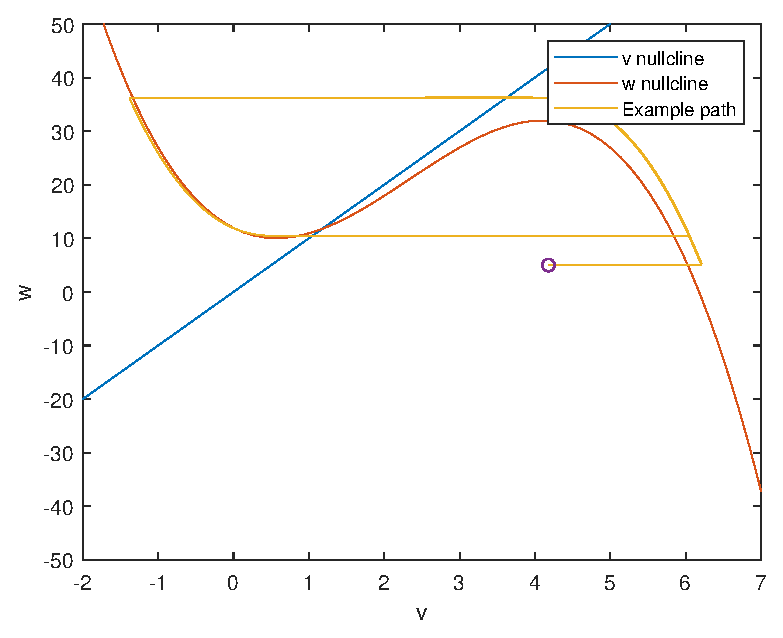
\includegraphics[width=0.6\linewidth]{A2Q2.eps}
		\caption{Example trajectory with $a = 6, b=10, A=1, \epsilon = 0.01$}
		\label{fig:q2}
	\end{figure}

	%Q3
	\item 

	\begin{enumerate}
		%Q3a
		\item As stated in the question: this is an age system, so $n(t,a) \delta a$ is the number of people in ages $a, a+ \delta a$ at time $t$.  
		\begin{itemize}
			\item $\beta(a)$ is effectively a birth probability/number for individuals at age $a$, i.e. the number of individuals that an individual at age $a$ will reproduce (with age $0$). 
			\item $B(t)$ is the convolution integral of $\beta * n$. It takes the integral of the birth probability with the number of individuals at all ages. It is the number of individuals born (i.e. age $0$) at time $t$.
		\end{itemize}
		%Q3b 
		\item First note:
		\[\odd Nz = \dd Na \dd az + \dd Nt \dd Nt = \dd Na + \dd Nt\]

		The equation along the curves $n(t,a) = n(t(z),a(z)) = N(z)$ 
		\begin{align*}
			\dd nt + \dd na = -\mu(a) n \\
			\dd Nt + \dd Na = - \mu(a) N \\
			\odd Nz= -\mu(a) N \\
		\end{align*}

		%Q3c 
		\item 
		\begin{enumerate}
			%Q3ci
			\item Integrating $(3)$ gives
			\begin{align*}
				\dd tz = 1,& \qquad \dd az =1\\
				t = z + t_0,&\qquad a = z + a_0\\
				t = z,& \qquad a = z + \theta\\
			\end{align*}
			$z=0$ gives $t=0$ and $a = \theta$.

			%apparently i have to sketch some of these curves?

			%Q3cii 
			\item 
			\begin{align*}
				\odd Nz &= - \mu(a) N\\
				\frac1N \odd Nz &= - \mu(z+\theta)\\
				\log N &= \int_0^z -\mu(\tau+\theta) d \tau\\
				N &= e^{C} \exp\left\{-\int_0^z \mu(\tau+\theta) d \tau\right\}
				N &= e^{C} \exp\left\{-\int_\theta^{z+\theta} \mu(\tau) d \tau\right\}
			\end{align*}
			So the $z=0$ condition is the $N(0) = n(0,\theta) = F(\theta)$
			Hence
			\begin{align*}
				N(0) &= e^{C} \exp\left\{-\int_\theta^{\theta} \mu(\tau) d \tau\right\}\\
				F(\theta)&= e^C \exp\{0\}\\
				\implies e^C &= F(\theta)
			\end{align*}
			\[N(z) = F(\theta) \exp\left\{-\int_\theta^{z+\theta} \mu(\tau) d \tau\right\}\]

			We can write $\theta = a-t$, and using $z+\theta = a$, we arrive at
			\[n(t,a) = F(a-t) \exp\left\{-\int_{a-t}^a \mu(\tau) d \tau\right\}\]

		\end{enumerate}

		%Q3d
		\item 
		\begin{enumerate}
			%Q3di
			\item Again, integrating $(3)$
			\begin{align*}
				\dd tz = 1,& \qquad \dd az =1\\
				t = z + t_0,&\qquad a = z + a_0\\
				t = z + \theta,& \qquad a = z\\
			\end{align*}
			%Q3dii 
			\item 
			\begin{align*}
				\odd Nz &= - \mu(a) N\\
				\frac1N \odd Nz &= - \mu(z)\\
				\log N &= \int_0^z -\mu(\tau) d \tau\\
				N &= e^{C_2} \exp\left\{-\int_0^{z} \mu(\tau) d \tau\right\}
			\end{align*}
			The $z=0$ condition instead gives $N(0) = n(\theta,0) = B(\theta)$, 

			\begin{align*}
				N(0) &= e^{C_2} \exp\left\{-\int_0^{0} \mu(\tau) d \tau\right\}\\
				B(\theta) &= e^{C_2} e^0\\
				\implies e^{C_2} &= B(\theta)
			\end{align*}
			And hence
			\[N = B(\theta) \exp\left\{-\int_0^{z} \mu(\tau) d \tau\right\}\]
			Then, using 
			\[t-a = z+\theta - z = \theta, \quad \text{and}, \quad a = z\]
			We get
			\[N(z) = B(t-a) \exp \left\{-\int_{0}^a \mu(\tau) d \tau\right\}\]
			And hence
			\[n(t,a) = B(t-a) \exp\left\{-\int_{0}^a \mu(\tau) d \tau\right\}\]

		\end{enumerate}
		%Q3e
		\item Using the definition of $B$:
		And the fact that
		\[n(t,a) = \begin{cases}
			F(a-t) \exp\left\{-\int_{a-t}^a \mu(\tau) d \tau\right\} & 0<t < a\\
			B(t-a) \exp\left\{-\int_{0}^a \mu(\tau) d \tau\right\}, & t> a	
		\end{cases}\]
		\begin{align*}
			B(t) &= \int_0^\infty \beta(a) n(t,a) da\\
			&= \int_0^\infty \beta(\tau) n(t,\tau) d \tau\\
			&= \int_0^t \beta(\tau) n(t,\tau) d \tau + \int_t^\infty \beta(\tau) n(t,\tau) d \tau\\
			B(t) &= \int_0^t \beta(\tau) B(t- \tau) \exp\left\{-\int_{0}^\tau \mu(q) d q\right\} d \tau + \int_t^\infty  \beta(\tau)F(\tau-t) \exp\left\{-\int_{\tau - t}^\tau \mu(\tau) d \tau\right\}  d \tau \\
		\end{align*}
	\end{enumerate}

	%Q4
	\item 
	\begin{enumerate}
		%Q4a
		\item 
		The steady state distribution obeys $\dd ct = 0$
		\begin{align*}
			D \ddn cx2 - kc = 0\\
			\ddn cx2 = \frac kD c
		\end{align*}
		Given that $kD > 0$, 
		\[c(x) = Ae^{\sqrt{kD} x} + Be^{-\sqrt{kD} x}\]
		To satisfy the two BCs:
		\begin{align*}
			c(0) = c_0 = A+B\\
			\dd cx\pipe_L = 0 = \sqrt{\frac{k}{D}}\left(Ae^{\sqrt{k/D} L} + Be^{-\sqrt{k/D} L}\right)\\
			0 = Ae^{\sqrt{k/D} L} + Be^{-\sqrt{k/D} L}\\
			B =- Ae^{2\sqrt{k/D} L}\\
			\implies A - Ae^{2\sqrt{k/D} L} = c_0\\
			A = \frac{c_0}{1 -e^{2\sqrt{k/D} L}}
		\end{align*}
		\[c(x) = \frac{c_0}{1 -e^{2\sqrt{k/D} L}} \left(e^{\sqrt{k/D} x} - e^{2\sqrt{k/D} L} e^{-\sqrt{k/D} x}\right) \]
		%Q4b 
		\item 
		\begin{align*}
			c = \theta\\
		\frac{c_0}{1 -e^{2\sqrt{k/D} L}} \left(e^{\sqrt{k/D} x_\theta} - e^{2\sqrt{k/D} L} e^{-\sqrt{k/D} x_\theta}\right) = \theta\\
		e^{\sqrt{k/D} x_\theta} - e^{2\sqrt{k/D} L} e^{-\sqrt{k/D} x_\theta} = \frac{\theta (1 -e^{2\sqrt{k/D} L})}{c_0}\\
		e^{\sqrt{k/D} x_\theta} - e^{\sqrt{k/D} (2L-x_\theta)} = \frac{\theta (1 -e^{2\sqrt{k/D} L})}{c_0}\\
		\end{align*}
		$x_\theta$ is the solution to this expression.

		%Q4c 
		\item If we write the equation as:
		\begin{align*}
		e^{-2\sqrt{k/D} L} e^{\sqrt{k/D} x_\theta} - e^{-\sqrt{k/D} x_\theta} = e^{-2\sqrt{k/D} L} \frac{\theta (1 -e^{2\sqrt{k/D} L})}{c_0}\\		
		e^{-2\sqrt{k/D} L} e^{\sqrt{k/D} x_\theta} - e^{-\sqrt{k/D} x_\theta} =  \frac{\theta (e^{-2\sqrt{k/D} L} - 1)}{c_0}\\		
		\end{align*}
		Sending $L \to \infty$, we get $e^{-L} \to 0$. So the equation becomes
		\begin{align*}
			-e^{-\sqrt{k/D} x_\theta} = -\theta/c_0\\
			e^{-\sqrt{k/D} x_\theta} = \theta/c_0\\
			-\sqrt{k/D}x_\theta = \log(\theta/c_0)\\
			x_\theta \to \frac{\log(c_0/\theta)}{\sqrt{k/D}}\\
			x_\theta \to \sqrt{\frac{D}{k}}\log(c_0/\theta)\\
		\end{align*}

		So when the column is infinitely long, we find that the distance $x_\theta$, where the cells become able to divide relates to the chemical concentration at the bottom of the column, the threshold $\theta$, the rates of diffusion and chemical consumption.  The ratio of diffusion to consumption, and bottom concentration to 

		$x_{\theta}$ will be the point where cells can no longer divide. Hence it makes sense that it increases with diffusion and base nutrient $c_0$, and similarly how it decreases with consumption rate and threshold $\theta$.

	\end{enumerate}
	%Q5
	\item 
	\begin{enumerate}
		%Q5a
		\item 
		And note
		\[\dd{}x = \dd{z}{x} \dd{}z\]
		% \[\dd Nz = \dd Nx \dd xz + \dd Nt \dd tz = \dd Nx + \dd Nt\]
		\[\dd Nt = \odd Nz \dd z t = -c\odd Nz = -cN'  \]
		\[\dd Nx = \odd Nz \dd z x = \odd Nz = N'\]
		And apply this to the equation:
		\begin{align*}
		\dd nt &= \dd{}x\left(n\dd{n}x\right) +  n(1-n)\\
		-c N' &= \odd{}z\left(NN'\right) + N(1-N)\\
		-c N' &= \left(N' \right)^2 + N N'' + N(1-N)\\
		N N'' &= -cN' - N'^2  - N(1-N)\\
		N'' &= -\frac{N'}{N} \left(c + N'\right) + N-1
		\end{align*}
		

		Letting $P(z) = N'(z) = \odd Nz$, gives the system
		\begin{align*}
			N'(z) &= P(z)\\
			P'(z) &= - \frac{P(z)}{N(z)} \left(c + P(z)\right) + N(z) - 1
		\end{align*}

		%Q5b 
		\item Make the change of variables on $z$:
		\[\zeta = \int_0^z \frac{1}{N(\eta)} d \eta\]
		\begin{align*}
			\dd{}z N(z) = \dd{N}\zeta \frac{1}{N(z)}\\
			N(z) \dd{N(z)}z  = \dd{N(\zeta)}\zeta\\
			N(z) P(z) = P(\zeta)
		\end{align*}
		so that 
		%allegedly
		\begin{align*}
			N' &= NP\\
			P' &= - P\left(c + P\right) + N(N - 1)
		\end{align*}

		Clearly the $N$ nullclines are for $P = 0$ and $N=0$
		
		$P$ nullclines with $P = 0$:
		\begin{align*}
			  - P\left(c + P\right) + N(N - 1) = 0\\
			 0\left(c + 0\right) +N(N - 1) = 0\\
			 N - 1 = 0, \quad N = 0\\
			 \implies N = 1, 0 
		\end{align*}

		Nullclines of the second equation with $N = 0$:
		\begin{align*}
			- P\left(c + P\right)= 0\\
			P = 0, \quad P = -c
		\end{align*}
		But $(0,0)$ is already a fixed point. Hence the fixed points are
		\[(N,P) = \begin{cases}
			(1,0)\\
			(0,0)\\
			(0,-c)			
		\end{cases}\]

		Figure~\ref{fig:Q5} shows these points for the non-transformed system. Ignoring the vertical blue line which relates to numerical instability.
		\begin{figure}[tb]
			\centering
			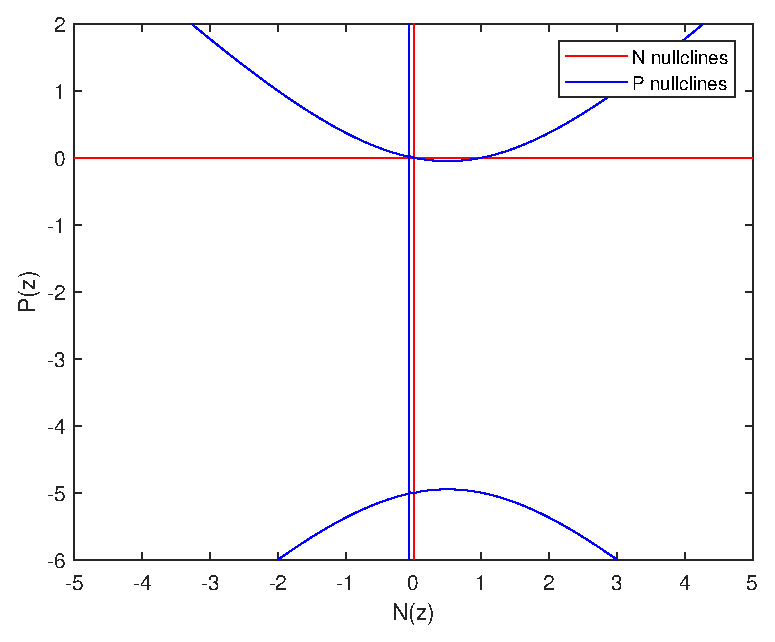
\includegraphics[width =0.6\linewidth]{A2Q5.eps}
			\caption{Plot of nullclines for $c = 5$}
			\label{fig:Q5}
		\end{figure}

		\clearpage
		%Q5c
		\item Typo in this question - should be $N(z)$ against $z$. Noting that $N$ is non-negative. Shown in figure~\ref{fig:sketch}. Both trajectories move from the point $(1,0)$ towards the respective other fixed points
		\begin{figure}[h]
			\centering
			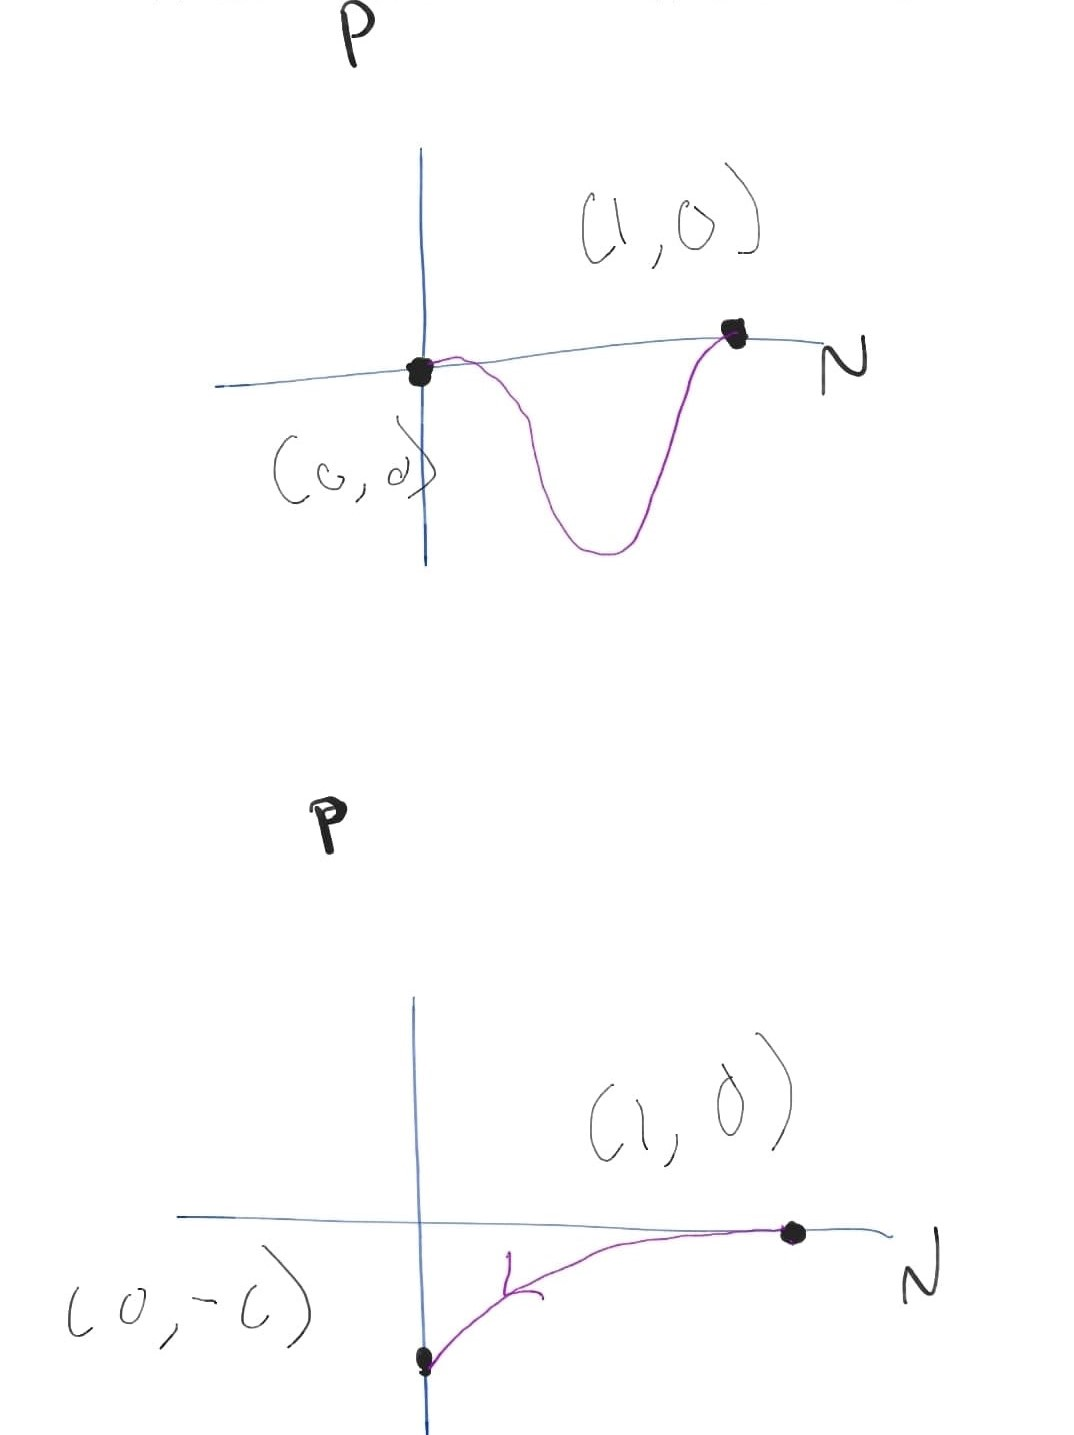
\includegraphics[width = 0.7\linewidth]{sketch.jpg}
			\caption{A pair of possible trajectories allowing for solutions to the system}
			\label{fig:sketch}
		\end{figure}

		%Q5d 
		\item 
		
		The algebra should be nicer if I go in terms of $N'$
		\begin{align*}
			N''(z) &= \dd{}z c(N(z) - 1) = c N '\\
			N'(z) &= c(N(z) - 1) \implies N = \frac{N'}{c} + 1
		\end{align*}
		\begin{align*}
			-cN' &= (N')^2 + N N'' + N(1-N)\\
			-cN' &= (N')^2 + cN'(\frac{N'}{c} + 1) - \frac{N'}{c}(\frac{N'}{c} + 1)\\
			-cN' &= (N')^2 + (N')^2 + cN' - \frac{(N')^2}{c^2} - \frac{N'}{c}\\
			-c &= N' + N' + c - \frac{N'}{c^2} - \frac{1}{c}\\
			0 &= 2N' + 2c - \frac{N'}{c^2} - \frac{1}{c}\\
			0 &= N'\left(2 - \frac{1}{c^2}\right) + c\left(2 - \frac{1}{c^2}\right)
		\end{align*}
		For non-trivial solutions, we require the parts in brackets to be zero.
		Hence
		\begin{align*}
			2 - \frac1{c^2} &= 0 \\
			c^2 = \frac12\\
			c = \pm \frac{1}{\sqrt{2}}
		\end{align*}
		And since $c > 0$, 
		\[\boxed{c = \frac{1}{\sqrt{2}}}\]
		
		The particular solution to the system:
		\begin{align*}
			P(z) =N'(z) &= c(N(z) - 1)\\
			\implies N(z) &= k e^{cz} + 1\\
		\end{align*}
		For a constant $k$.

		To satisfy the condition
		\begin{align*}
			N(z_c) &= 0 \\
			k e^{cz_c} + 1 &=0\\
			k = -e^{-cz_c}
		\end{align*}

		Hence
		\[N = -e^{c(z-z_c)} + 1\]

		$z > z_c$ refers to $x - ct > z_c$, i.e. for early time, and positive position, the density of cells will be zero.

		Of course this solution doesn't account for the limitation that $N$ must be positive. Realistically it is given by:
		\[N(z) = \max\left\{0,-e^{c(z-z_c)} + 1\right\}\]

		This relates to the combination of the fixed point $(1,0)$ and path prior to this. The fixed point $(0,-c)$ is the only fixed point which allows the exponential decay while obeying the two solutions, given $N$ has to be positive. This means that at the point $N(z) = 0$, the slope is $0$. So $N(z)=0$ for all $z > z_c$. 
	\end{enumerate}
\end{enumerate}

\section*{Code}

\lstinputlisting{A2Code.m}

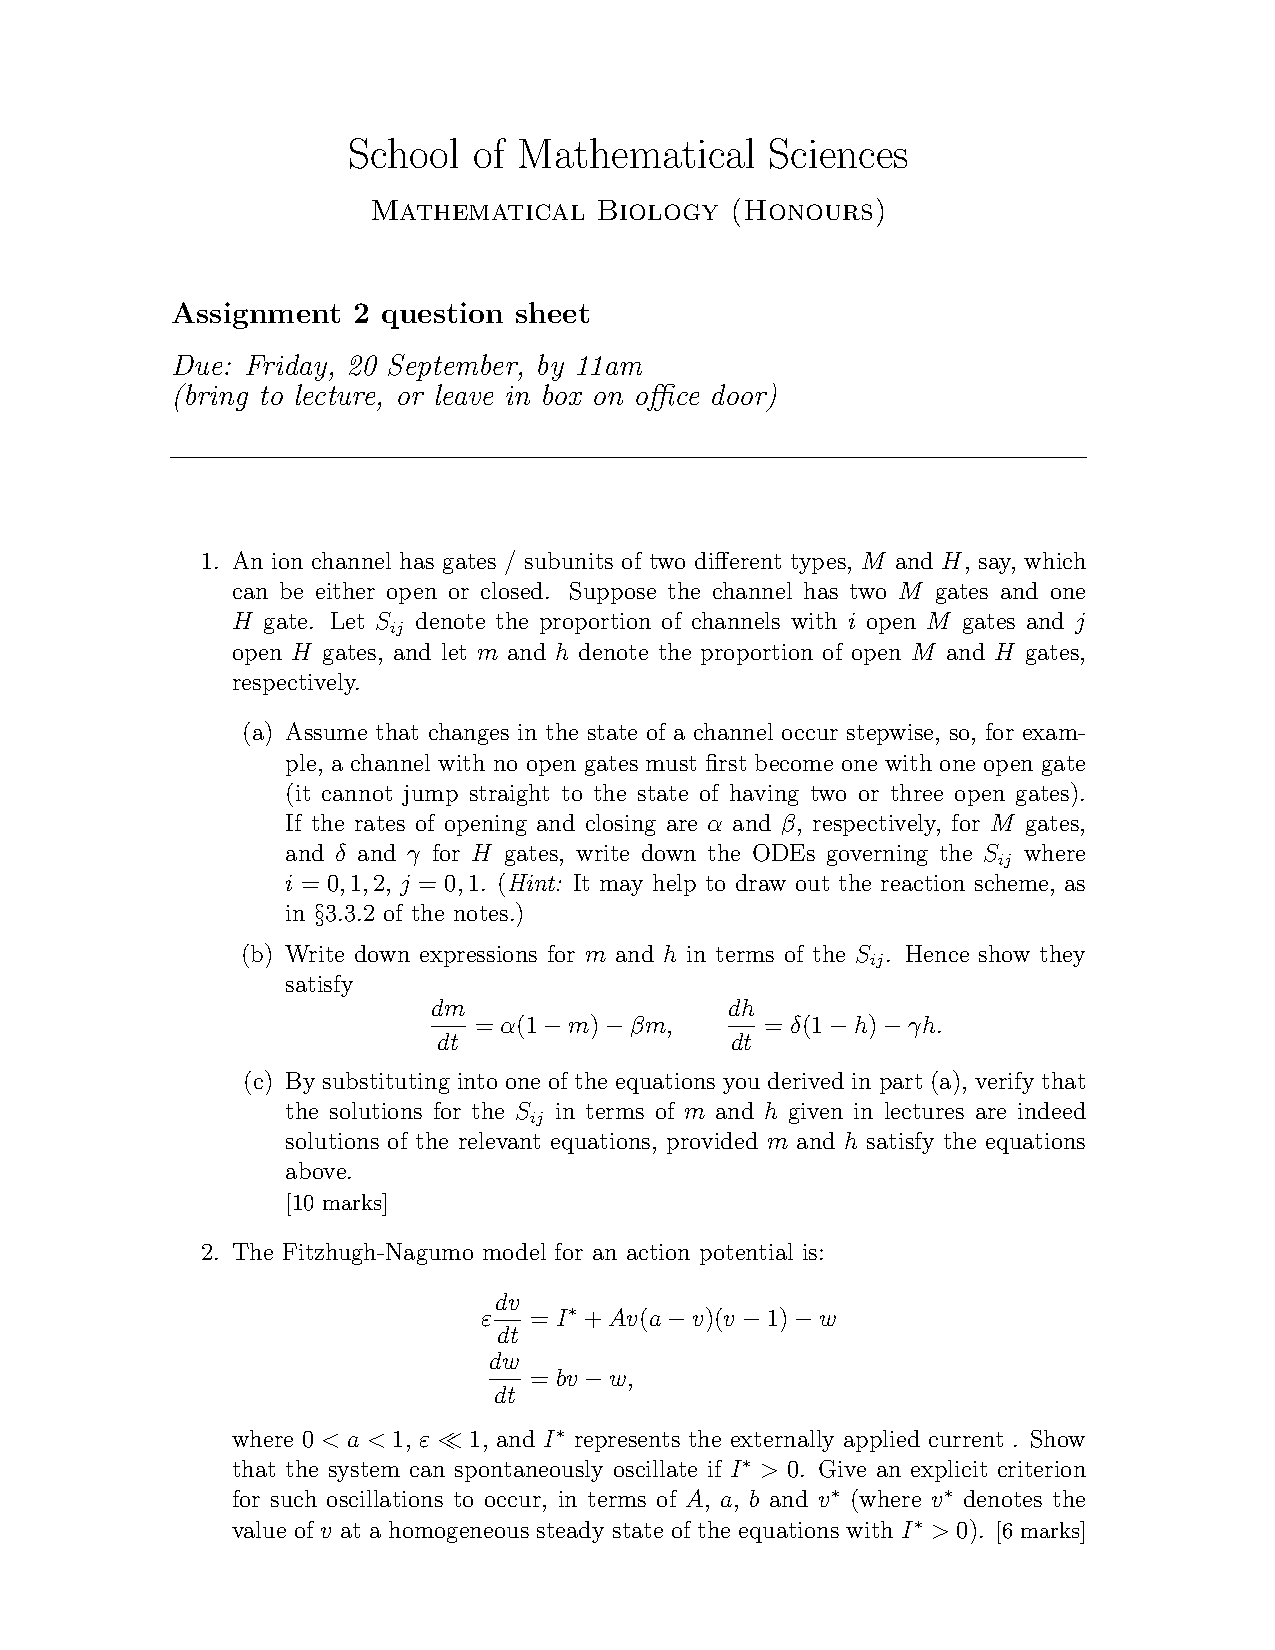
\includepdf[pages=1-]{A2_2019.pdf}


\end{document}

